\documentclass{homework}
% \usepackage{graphicx} % Required for inserting images
\usepackage{amsmath}
\usepackage{gensymb}
\usepackage{subfig}
\usepackage{float}

\class{ECEN 5417}
\title{Homework 3}
\author{Sean Jennings}
\date{October 9, 2023}

\begin{document}
\maketitle

Note: all numerical values are rounded to at most 4 significant figures upon display.
(Assume values displayed with less significant digits have trailing 0s.)

\section{Problem 3.2}
\begin{align*}
    \alpha &= N_1 / N_2 = \boxed{4.0} \\
    V_2 &= V_1 / \alpha = \boxed{250.0 \angle 0.0 \degree \V} \\
    I_2 &= I_1 \alpha = \boxed{20.0 \angle -30.0 \degree \A} \\
    Z_2 &= V_2 / I_2 = \boxed{12.5 \angled{30.0} \ohm = 10.83 + j 6.25 \ohm} \\
    Z_2' &= V_1 / I_1 = \alpha^2 Z_2 = \boxed{200 \angled{30.0} \ohm = 173.2 + j 100.0 \ohm} \\
\end{align*}

\section{Problem 3.4}
From the problem statement, we deduce:
\begin{align*}
    |S_2| &= 80\kVA \\
    pf &= 0.8 \\
    V_2 &= 230 \V \\
    \alpha &= \frac{V_{r,1}}{V_{r,2}} = 2400\V / 240 \V = 10
\end{align*}
Then, complex power from apparent power and power factor is:
\begin{equation*}
    S_2 = |S_2| \cdot (pf + j \sin(\arccos(pf)))
        = 80 \angled{36.87} \kVA = 64.0 + j 48.0 \kVA
\end{equation*}

\begin{letterenum}
    \item \begin{equation*}
        V_1 = \alpha V_2 = 2300. \V = \boxed{2.3 \kV}
    \end{equation*}
    \item \begin{equation*}
        Z_2 = |V_2|^2 / S_2^* = \boxed{661.2 \angled{36.87} \mohm} 
    \end{equation*}
    \item \begin{equation*}
        Z_2' = \alpha^2 Z_2 = \boxed{66.12 \angled{36.87} \ohm}
    \end{equation*}
    \item Since we assume the transformer is ideal, power is conserved.
    \begin{align*}
        S_1 &= S_2 \\
        P_1 &= \boxed{64.0 \kW} \\
        Q_1 &= \boxed{48.0 \kVAr}
    \end{align*}
\end{letterenum}

\section{Problem 3.8}
Inputs:
\begin{align*}
    V_{in} &= 18/\sqrt{2} \V \\
    R_1 &= 18 \text{ } \ohm \\
    R_2 &= 36 \text{ } \ohm \\
    R_3 &= 2 \text{ } \ohm \\
    R_4 &= 8 \text{ } \ohm \\
    \alpha &= 2 / 1
\end{align*}
To solve the circuit, we define rated power and voltage to be convenient
numbers and per-unitize.
Rated voltage, power, and impedance are given as follows.
Note that $X_r$ subscript of some quantity $X$ denotes $X$'s rated value.
\begin{align*}
    V_{r,1} &= 18 \V \\
    S_r &= 18^2 \VA \\
    Z_{r,1} &= V_{r,1}^2 / S_r = 1 \ohm \\
    Z_{r,2} &= Z_{r,1} / \alpha^2 = 0.25 \ohm
\end{align*}

Since the coil ratio of second transformer is the inverse of the first,
we use the rated impedance $Z_{r,1}$ and voltage $V_{r,1}$ as the rated
voltages for the output component of the circuit.

We now per-unitize:
\begin{align*}
    V_{in,pu} = V_{in} / V_{r,1} &= 0.7071 \\
    R_{1,pu} = R_1 / Z_{r,1} &= 18 \\
    R_{2,pu} = R_2 / Z_{r,1} &= 36 \\
    R_{3,pu} = R_3 / Z_{r,2} &= 8 \\
    R_{4,pu} = R_4 / Z_{r,1} &= 8 \\
\end{align*}

We now solve the circuit by calculating parallel/series impedances
and using the voltage divider law. $R_{p,pu}$ is the per-unit
equivalent resistance of the two parallel branches containing
$R_1$, $R_2$, and $R_3$. $V_2$ is the intermediate voltage at the
node above this branch.

\begin{align*}
    R_{p,pu} = \biggl(\frac{1}{R_{2,pu}} + \frac{1}{R_{3,pu} + R_{4,pu}}\biggr)^{-1}
        &= 11.08 \\
    V_{2,pu} = \frac{R_{p,pu}}{R_{1,pu} + R_{p,pu}} V_{in,pu} &= 0.2694 \\
    V_{out,pu} = \frac{R_{4,pu}}{R_{3,pu} + R_{4,pu}} V_{2,pu} &= 0.1347 \\
\end{align*}

Converting back to non-per-unit values and converting back from RMS to instantaneous
gives:
\begin{equation*}
    V_{out,pp} = \sqrt{2} V_{out} = \sqrt{2} V_{out,pu} V_{r,1} = 3.429 \V
\end{equation*}
So, as an instantaneous power
\begin{equation*}
    \boxed{v_{out}(t) = 3.429 \sin(10t) \V}
\end{equation*}

\section{Problem 3.14/19}
\subsection{Part 1}

Inputs:
\begin{align*}
    Z_1 &= 1 + j2.0 \ohm \\
    Z_2 &= 1 + j2.5 \ohm \\
    S_r &= 50 \kVA \\
    pf &= 0.8 \text{ lagging} \\
    V_{r,1} &= 2400 \V \\
    V_{r,2} &= 240 \V \\
\end{align*}

$Z_2$ is the transformer impedance, and $Z_1$ is the feeder-side
series impedance, as shown in Figure \ref{fig:circuit_314}. The AC
circuit analysis proceeds as follows:

\begin{center}
    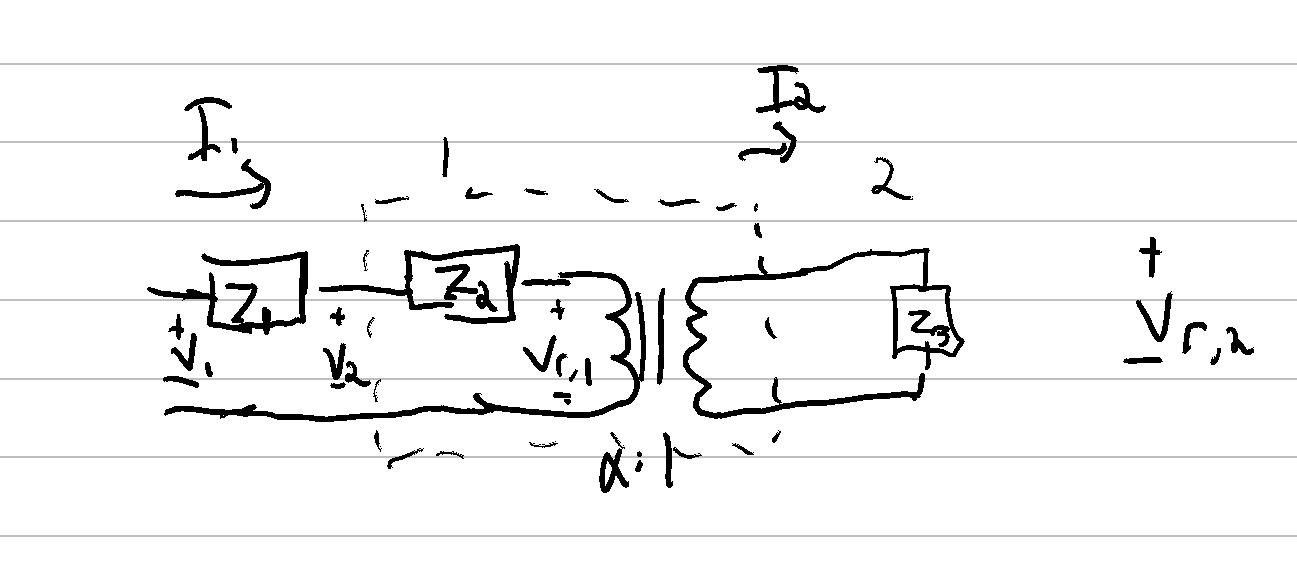
\includegraphics[width=0.5\linewidth]{Images/problem_3_14.png}
    \captionof{figure}{Circuit problem 3.14}
    \label{fig:circuit_314}
\end{center}

\begin{align*}
    S_3 &= S_r(pf + j(\sin(\arccos(pf)))) = 50 \angled{36.87} \kVA \\
    I_2 &= S_3^* / V_3 \\
    I_1 &= \frac{I_2}{\alpha} = \frac{S_3^*}{\alpha V_3}
        = \frac{S_3^*}{V_{r,1}} = 20.83 \angled{-36.87} A \\
    V_2 &= V_{r,1} + Z_2 I_1 = \boxed{2448. \angled{0.6826} \V} \\
    V_1 &= V_2 + Z_2 I_1 = \boxed{2490. \angled{1.151} \V} \\
    S &= S_3 + (Z_1 + Z_2) |I_1|^2 = 51.88 \angled{38.02} \kVA \\
    P &= \boxed{40.87 \kW} \\
    Q &= \boxed{31.95 \kVAr}
\end{align*}

Then the requested quantities are
\begin{letterenum}
    \item given by $V_2$,
    \item given by $V_1$,
    \item and given by $P$ and $Q$
\end{letterenum}

\subsection{Part 2}
We repeat the computation with via per-unitization. The equivalent
per-unitized circuit is shown in figure \ref{fig:circuit_319}

\begin{center}
    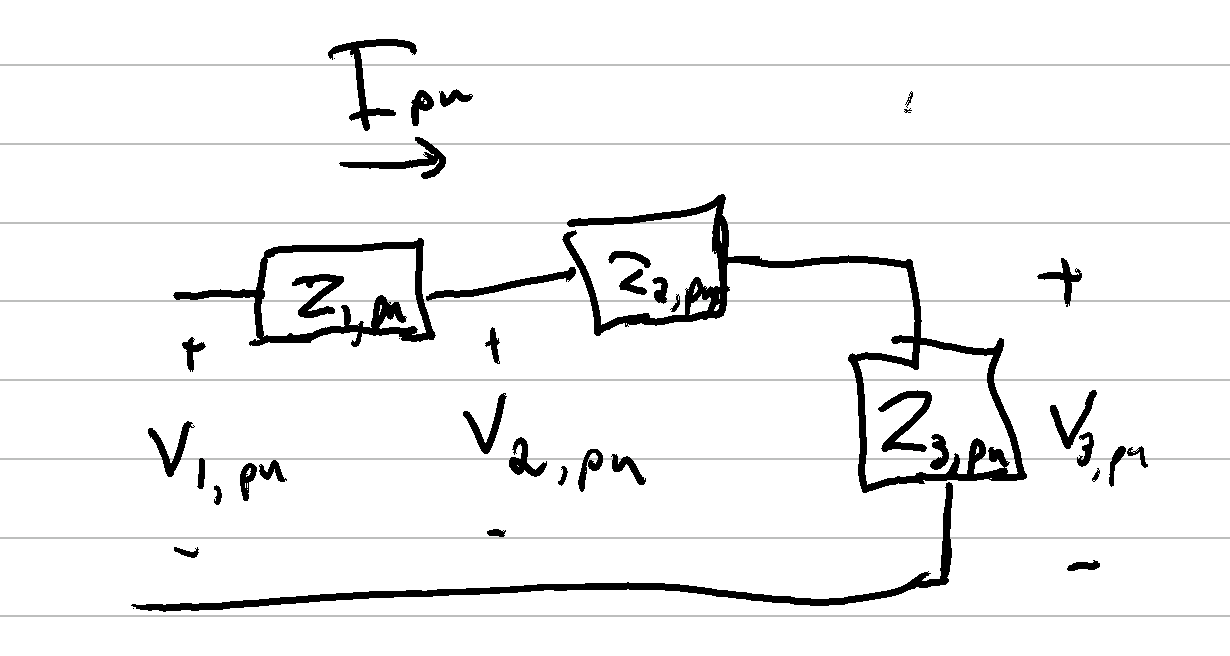
\includegraphics[width=0.5\linewidth]{Images/problem_3_19.png}
    \captionof{figure}{Per-unitized equivalent}
    \label{fig:circuit_319}
\end{center}

\begin{align*}
    Z_{r,1} &= V_{r,1}^2 / S_r = 115.2 \ohm \\
    Z_{1,pu} &= Z_1 / Z_{r,1} = 0.01941 \angled{63.43} \\
    Z_{2,pu} &= Z_2 / Z_{r,1} = 0.02337 \angled{68.2} \\
    V_3 &= V_{r,2} \\
    V_{3,pu} &= V_3 / V_{r,2} = 1 \\
    S_{3,pu} &= S_3 / S_r = 1 \angled{36.87} \\
    I_{pu} &= S_{3,pu}^* / V_{3,pu} = S_{3,pu}^* = 1 \angled{-36.87} \\
    V_{2,pu} &= 1 + Z_{2,pu} I_{pu} = \boxed{1.02 \angled{0.6826}} \\
    V_{1,pu} &= 1 + (Z_{1,pu} + Z_{2,pu}) I_{pu} = \boxed{1.038 \angled{1.151}} \\
    S_{pu} &= S_{1,pu} + S_{2,pu} + S_{3,pu} \\
        &= (Z_{1,pu} + Z_{2,pu}) |I_{pu}|^2 + S_{3,pu} = \boxed{1.038 \angled{38.02}}
\end{align*}

Validating with numbers from part 1.

\begin{align*}
    V_2 = V_{2,pu} V_{r,1} = 2448. \angled{0.6826} \V \\
    V_1 = V_{1,pu} V_{r,1} = 2490. \angled{1.151} \V \\
    S = S_{pu} S_r = 51.88 \angled{38.02} \kVA
\end{align*}
Equivalent $P$ and $Q$ clearly follow from an equivalent complex power $S$.

\section{Problem 3.23}
Input:
\begin{align*}
    S_r = 100 \MVA \\
    Z_{\ell_1} = 48.4 \ohm \\
    Z_{\ell_2} = 65.43 \ohm \\
    |S_L| = 57 \MVA \\
    pf = 0.6 \\
    V_L = 10.45 \kV 
\end{align*}

Figure \ref{fig:impedance_diagram} shows the impedance diagram for the given
one-line diagram. Per-unit values for $Z_G$, $Z_M$, $Z_T1$, $Z_T2$,
$Z_T3$, and $Z_T4$ are found from the provided table. 

\begin{center}
    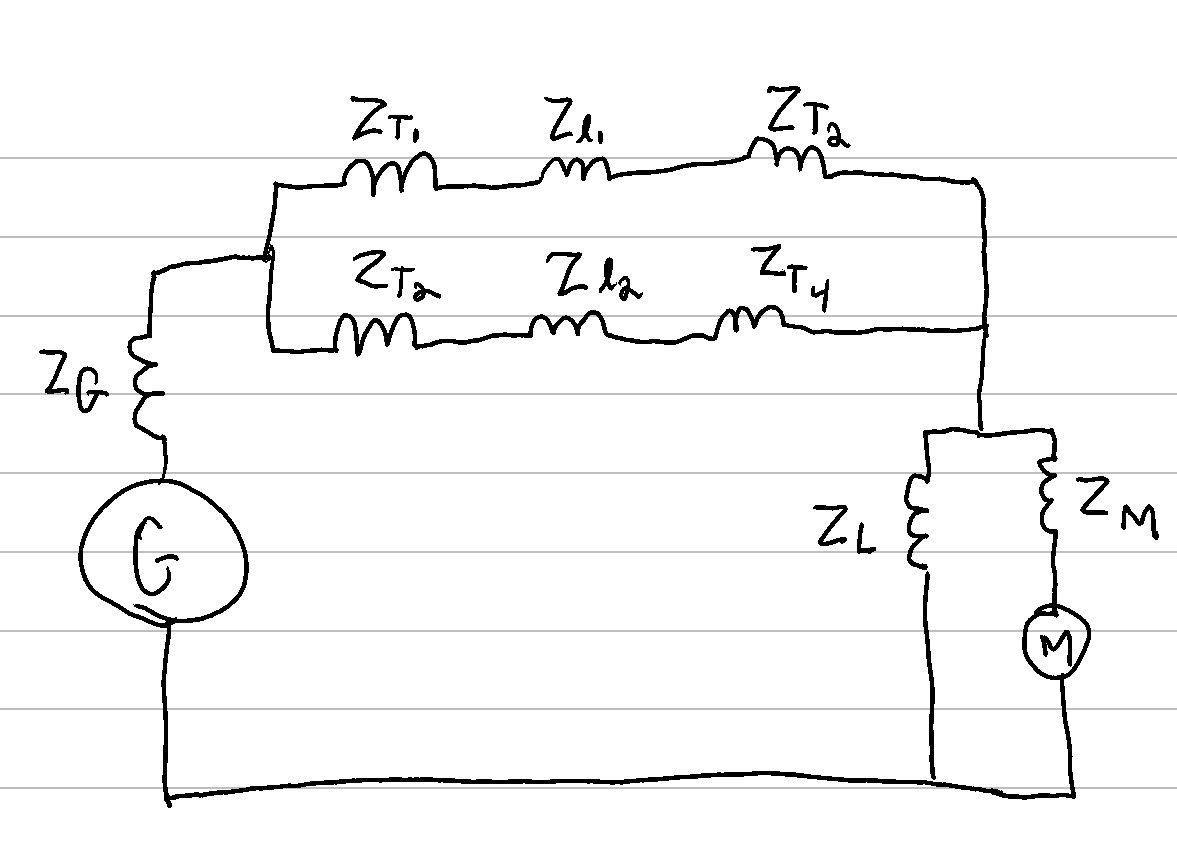
\includegraphics[width=0.5\linewidth]{Images/problem_3_23.png}
    \captionof{figure}{Impedance Diagram}
    \label{fig:impedance_diagram}
\end{center}

Since the rate voltage at bus 1 is defined at the rated voltages of $T1$ and
$T_3$ and all transformers operate at rated values, we deduce the
rated voltages for line 1, line 2, and bus 4 from the transformer ratings:
\begin{align*}
    V_{r,\ell_1} = 220 \kV \\
    V_{r,\ell_2} = 110 \kV \\
    V_{r,4} = 11 \kV
\end{align*}
Line impedance can then be calculated as follows
\begin{align*}
    Z_{i,pu} &= \frac{Z_i}{Z_{i,r}} = \frac{Z_i S_r}{V_{i,r}^2}
        \qquad i \in \{\ell_1, \ell_2\} \\
    Z_{\ell_1,pu} &= \boxed{j 0.1} \\
    Z_{\ell_2,pu} &= \boxed{j 0.5407}
\end{align*}
The comlex power drawn by the load, and the load's per-unit impedance
follow:
\begin{align*}
    S_L = |S_L| (pf + j \sin(\arccos(pf))) = 57 \angled{53.13} \MVA \\
    Z_L = V_L^2 / S_L^* \\
    Z_{r,4} = V_{r,4}^2 / S_r \\
    Z_{L,pu} = \frac{Z_L}{Z_{r,4}} = \frac{V_L^2 S_r}{V_{r,4}^2 S_L^*} = \boxed{
        1.583 \angled{53.13}
    }
\end{align*}


\section{Problem 8.10}
Input:
\begin{align*}
    V_{ag} = 280 \angled{0} \\
    V_{bg} = 250 \angled{-110} \\
    V_{cg} = 290 \angled{130} \\
\end{align*}

\begin{letterenum}
    \item Let $V_{Lg} = [V_{ag}, V_{bg}, V_{cg}]^T \in \C^3$ be the 
    phase voltages. Let $A$ be the matrix representation of the sequence basis
    w.r.t the standard basis of $\C^3$. That is,
    \begin{equation}
        A = \mat{
            1 & 1 & 1 \\
            1 & a^2 & a \\
            1 & a & a^2 \\
        }
    \end{equation}
    where $a = 1 \angled{120}$. Then, the sequence components are given by
    \begin{equation*}
        V_{s,Lg} = \mat{
            V_{Lg0} \\ V_{Lg1} \\ V_{Lg2}
        } = A^{-1} V_{Lg} = \boxed{\mat{
            5.039 \angled{-57.65} \\
            272.4 \angled{6.59} \\
            27.82 \angled{-76.05} \\
        } \V}
    \end{equation*}
    Note: we wil use the subscript $V_s \in \C^3$ to denote the sequence components
    of vector $V \in \C^3$.

    \item Line-to-line voltage can also be computed by a matrix multiplication.
    Let $B$ be the matrix:
    \begin{equation}
        B = \mat{
            1 & -1 & 0 \\
            0 & 1 & -1 \\
            -1 & 0 & 1
        }
    \end{equation}
    Then,
    \begin{equation*}
        V_{LL} = \mat{
            V_{ab} \\ V_{bc} \\ V_{ca}
        } = \mat{
            V_{ag} - V_{bg} \\ V_{bg} - V_{cg} \\ V_{cg} - V_{ag} \\
        }= B V_{Lg} = \boxed{\mat{
            434.5 \angled{32.73} \\
            468.1 \angled{-77.55} \\
            516.6 \angled{154.5} \\
        } \V}
    \end{equation*}
    \item Again, apply $A^{-1}$ to obtain the sequence components of line-to-line voltages
    (in other words, representation of $V_{LL}$ in the sequence basis):
    \begin{equation*}
        V_{s,LL} = \mat{
            V_{LL0} \\ V_{LL1} \\ V_{LL2}
        } = A^{-1} V_{LL} = \boxed{\mat{
            0 \\
            471.8 \angled{36.59} \\
            48.19 \angled{-106} \\
        } \V}
    \end{equation*}
    To show desired equality between sequence and standard representations of
    line-to-line voltages, we first note that $V_{LL} = B V_{Lg} = BA V_{s,Lg}$.
    Subsituting into the previous equation yields $V_{s,LL} = A^{-1} BA V_{s,Lg}$.
    Therefore, we compute $A^{-1} BA$ as follows
    \begin{align*}
        A^{-1}BA
            &= \frac{1}{3} \mat{
                1 & 1 & 1 \\
                1 & a & a^2 \\
                1 & a^2 & a \\
            } \mat{
                1 & -1 & 0 \\
                0 & 1 & -1 \\
                -1 & 0 & 1 \\
            } \mat{
                1 & 1 & 1 \\
                1 & a^2 & a \\
                1 & a & a^2 \\
            } \\
            &= \frac{1}{3} \mat{
                0 & 0 & 0 \\
                1-a^2 & a-1 & a^2 - a \\
                1-a & a^2 - 1  & a - a^2 \\
            } \mat{
                1 & 1 & 1 \\
                1 & a^2 & a \\
                1 & a & a^2 \\
            } \\
            &= \frac{a-1}{3} \mat{
                0 & 0 & 0 \\
                a^2 & 1 & a \\
                -1 & -a^2  & -a \\
            } \mat{
                1 & 1 & 1 \\
                1 & a^2 & a \\
                1 & a & a^2 \\
            } \\
            &= \frac{a-1}{3} \mat{
                0 & 0 & 0 \\
                0 & 3a^2 & 0 \\
                0 & 0  & -3 \\
            } \\
            &= \mat{
                0 & 0 & 0 \\
                0 & 1 - a^2 & 0 \\
                0 & 0  & 1 - a \\
            }
    \end{align*}
    where we've made use of various properties of $a$, including $1 + a + a^2 = 0$
    and $a^3 = 1$. Since $1-a^2 = \sqrt{3} \angled{30}$ and $1-a = \sqrt{3} \angled{-30}$, 
    we obtain the desired equality
    \begin{equation*}
        V_{s,LL} = \mat{
            V_{s,LL0} \\ V_{s,LL1} \\ V_{s,LL2}
        }= A^{-1}BAV_{LL} = \mat{
            0 \\
            \sqrt{3} V_{LL1} \angled{30} \\
            \sqrt{3} V_{LL2} \angled{-30}
        }
    \end{equation*}
    Of course, we can also just plug in numbers into a computer... but the
    author finds that rather less illuminating.
\end{letterenum}


\section{Problem 8.13}
Input:
\begin{align*}
    I_{ab} = 10 \angled{0} \A \\
    I_{bc} = 15 \angled{-90} \A \\
    I_{ca} = 20 \angled{90} \A \\
\end{align*}

\begin{letterenum}
    \item Let $I_\Delta := [I_{ab}, I_{bc}, I_{ca}]^T \in \C^3$.
    We multiply again by $A^{-1}$ to obtain the sequence delta currents
    $I_{s,\Delta} := [I_{\Delta0}, I_{\Delta1}, I_{\Delta2}]^T$.
    \begin{align*}
        I_{s, \Delta} = A^{-1} I_\Delta = \boxed{\mat{
            3.727 \angled{26.57} \\
            13.47 \angled{-3.548} \\
            6.821 \angled{-173} \\
        }} \A
    \end{align*}

    \item Define the line current $I_L \in \C^3$ as the stack of the
    line currents $I_L := [I_a, I_b, I_c]^T$. Then, converting the
    current relations for the delta circuit into matrix form, we have
    \begin{align*}
        I_L = \mat{
            I_a \\ I_b \\ I_c
        } = \mat{
            I_{ab} - I_{ca} \\ I_{bc} - I_{ab} \\ I_{ca} - I_{bc}
        } = \mat{
            1 & 0 & -1 \\
            -1 & 1 & 0 \\
            0 & -1 & 1 \\
        } I_\Delta = B^T I_\Delta
        &= \boxed{\mat{
            22.36 \angled{-63.43} \\
            18.03 \angled{-123.7} \\
            35. \angled{90.} \\
        } \A}
    \end{align*}
    where $B^T$ is the transpose of the matrix $B$ from the previous
    problem.
    
    \item We now decompose the line current $I_L$ into its sequence
        components $I_{s, L} := [I_{L0}, I_{L1}, I_{L2}]^T \in \C^3$
        by multiplying by $A^{-1}$.
        \begin{equation}
            I_{s,L} = A^{-1} I_L = \boxed{\mat{
                0 \\
                23.32 \angled{-33.56} \\
                11.82 \angled{-143.0} \\
            } \A}
        \end{equation}

        To verify the general relation between the sequence components of
        the delta and line currents, we first note a few preliminary facts:
        \begin{itemize}
            \item $a$ and $a^2$ are conjugates of each other:
                \begin{equation}
                    a^* = a^2 \qquad (a^2)^* = a
                \end{equation}
            \item The conjugate of $A$ is thus given by:
            \begin{equation}
                A^* = \mat{
                    1 & 1 & 1 \\
                    1 & a & a^2 \\
                    1 & a^2 & a \\
                } = 3A^{-1}
            \end{equation}
            \item $A$ and $A^{-1}$ are symmetric (i.e. $A^T = A$ and $A^{-1} = (A^{-1})^T$).
            \item The conjugate (Hermitian) transpose of $A^{-1}B^TA$ is given by:
            \begin{align*}
                (A^{-1}B^TA)^{T*} &= (ABA^{-1})^* \\
                    &= (3A^{-1})B(\frac{1}{3}A) \\
                    &= A^{-1}BA 
            \end{align*}
        \end{itemize}
        Now, analogous to the previous problem and using the previously derived
        expression for $A^{-1}BA$, we have
        \begin{align*}
            I_L &= A^{-1}B^TA I_\Delta  \\
                &= (A^{-1}BA)^{T*} I_\Delta \\
                &= \mat{
                    0 & 0 & 0 \\
                    0 & 1 - a^2 & 0 \\
                    0 & 0 & 1-a \\
                }^{T*} I_\Delta \\
                &= \mat{
                    0 \\
                    (1 - a) I_{\Delta1} \\
                    (1 - a^2) I_{\Delta2} \\
                } \\
                &= \mat{
                    0 \\
                    \sqrt{3} I_{\Delta1} \angled{-30} \\
                    \sqrt{3} I_{\Delta2} \angled{30} \\
                }
        \end{align*}
        completing the proof.
\end{letterenum}


\section{Problem 8.14}

Input:
\begin{align*}
    Z_y = 12 + j16 \ohm \\
    V_{ag} = 280 \angled{0} \V \\
    V_{bg} = 250 \angled{-110} \V \\
    V_{cg} = 290 \angled{130} \V \\
\end{align*}

Assume $Z_n >> Z_y$.

Figure \ref{fig:sequence_network} shows the sequence network diagram.
\begin{center}
    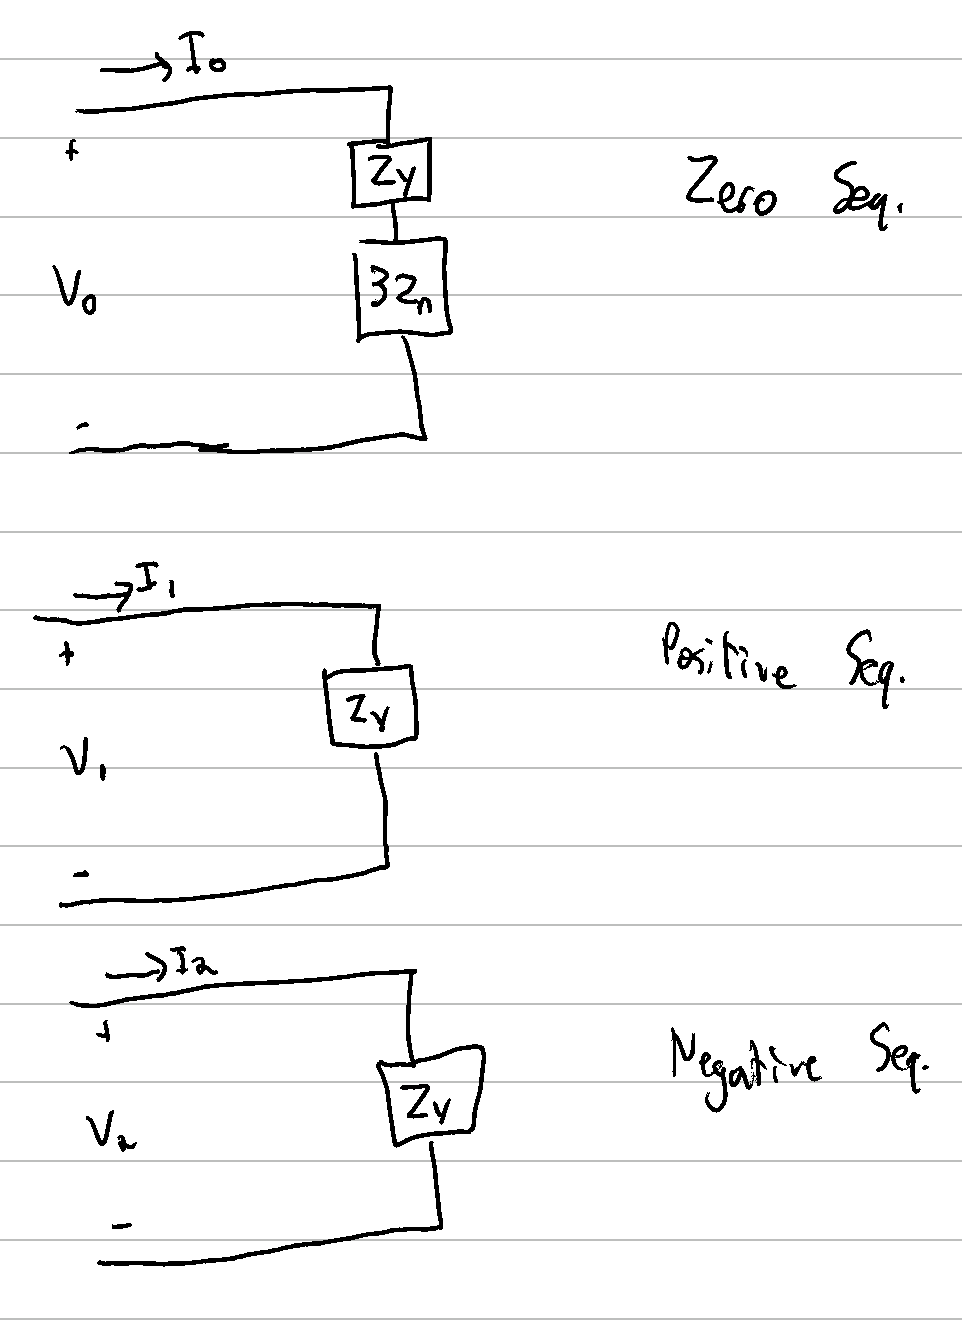
\includegraphics[width=0.5\linewidth]{Images/sequence_network.png}
    \captionof{figure}{Sequence network}
    \label{fig:sequence_network}
\end{center}

The computation then nicely simplifies by first converting
into the sequence coordinates. 

\begin{align*}
    V_s &= A^{-1} \mat{
        V_{ag} \\ V_{bg} \\ V_{cg}
    } = \mat{
        5.039 \angled{-57.65} \\
        272.4 \angled{6.59} \\
        27.82 \angled{-76.05} \\
    } \V \\
    I_s &= Z_s^{-1} V_s = \mat{
        \frac{1}{Z_y + 3Z_n} & 0 & 0 \\
        0 & \frac{1}{Z_y} & 0 \\
        0 & 0 & \frac{1}{Z_y}
    } V_s  \\
    &\approx \mat{
        0 & 0 & 0 \\
        0 & \frac{1}{Z_y} & 0 \\
        0 & 0 & \frac{1}{Z_y}
    } V_s \\
    &= \boxed{\mat{
        0 \angled{0} \\
        13.62 \angled{-46.54} \\
        1.391 \angled{-129.2} \\
    }} \A \\
    I & = A I_s = \boxed{\mat{
        13.86 \angled{-52.24} \\
        12.35 \angled{-164.1} \\
        14.75 \angled{76.74} \\
    } \A}
\end{align*}
Note: $I_s = [I_0, I_1, I_2]^T$ and $I = [I_a, I_b, I_c]^T$








\end{document}
